\chapter{Implementacija i korisničko sučelje}
		
		
		\section{Korištene tehnologije i alati}
		
		
			Komunikacija u timu ostvarena je korištenjem aplikacije WhatsApp \footnote{\url{https://www.whatsapp.com/}}. Kao sustav za upravljanje izvornim kodom korišten je Git \footnote{\url{https://git-scm.com/}}, a izvorni kod projekta dostupan je na Github \footnote{\url{https://github.com/}} web platformi . Za izradu dokumentacije korištena je distribucija markup jezika LaTeX MiKTeX \footnote{\url{https://miktex.org/}}  u kombinaciji s TeXstudio \footnote{\url{https://www.texstudio.org/}} radnom okolinom.
				
			Za izradu aplikacije koristila su se dva razvojna okruženja, Visual Studio Code\footnote{\url{https://code.visualstudio.com/}} za frontend i JetBrains IntelliJ IDEA \footnote{\url{https://www.jetbrains.com/idea/}} za backend. Visual Studio Code je radna okolina koju razvija i održava Microsoft, vrlo je fleksibilna te omogućava razvoj u širokom spektru jezika i tehnologija. JetBrains IntelliJ IDEA je razvojno okruženje specifično dizajnirano za rad s programskim jezikom Java, održava je tvrtka JetBrains koja je poznata po proizvodnji razvojnih okolina.
			
			Za izradu backenda korišten je programski jezik Java\footnote{\url{https://www.java.com/en/}} i radni okvir Spring \footnote{\url{https://spring.io/}}. Spring je radni okvir koji nudi gotova rješenja za mnoge često potrebne funkcionalnosti programskih sustava, time programerima omogućuje jednostavniji, brži i sigurniji razvoj aplikacija. 
			
			Za izradu frontenda korišten je programski jezik JavaScript\footnote{\url{https://developer.mozilla.org/en-US/docs/Web/javascript}} i biblioteka React\footnote{\url{https://react.dev/}}. React je biblioteka za razvoj korisničkih sučelja, u složenijim sustavima koristi se s drugim bibliotekama gdje služi kao temeljni sustav sučelja. React održava Facebook.
			
			Za izradu baze podataka korištena je implementacija SQL-a zvana PostgreSQL\footnote{\url{https://www.postgresql.org/}}. 
			
			Za skeniranje dokumenata i njihovo pretvaranje u txt datoteke korišten je OCR Tessaract.\footnote{\url{https://tesseract-ocr.github.io/tessdoc/Home.html}} Tessaract je projekt otvorenog izvornog koda kojeg održava zajednica volontera a omogućuje pretvorbu slika teksta u txt datoteke preko API-a.
			
			Za pohranu slika korištena je Googleova usluga Firebase. Firebase je web platforma za razvoj video igara i aplikacija koja nudi gotova rješenja i infrastrukture. U sklopu ovog projekta korištena je za pohranu slika jer druge usluge nisu dopuštale dovoljno prostora.
			
			Za objavu dokumenata na internetskim mrežama korišten je API društvene mreže Facebook.
			
			Kao platformu za puštanje u pogon odabrane je Render \footnote{\url{https://render.com/}} Render je WEB platforma specifično dizajnirana za puštanje aplikacija u pogon. Render pruža jednostavnu i učinkovitu infrastrukturu u oblaku zajedno s ograničenom memorijom za bazu podataka. Render održava istoimena tvrtka. Kako bi se zadovoljio format u kojem Render očekuje aplikaciju za puštanje u pogon dodatno se koristio alat Docker \footnote{\url{https://www.docker.com/}}. Docker je alat za pakiranje aplikacije sa svim potrebnim sredstvima za pokretanje aplikacije, time se postiže mogućnost pokretanja aplikacije na širokom spektru arhitektura. Docker također održava istoimena tvrtka.
			
		
	
		\section{Ispitivanje programskog rješenja}
			
			\subsection{Ispitivanje komponenti}
			\textit{Potrebno je provesti ispitivanje jedinica (engl. unit testing) nad razredima koji implementiraju temeljne funkcionalnosti. Razraditi \textbf{minimalno 6 ispitnih slučajeva} u kojima će se ispitati redovni slučajevi, rubni uvjeti te izazivanje pogreške (engl. exception throwing). Poželjno je stvoriti i ispitni slučaj koji koristi funkcionalnosti koje nisu implementirane. Potrebno je priložiti izvorni kôd svih ispitnih slučajeva te prikaz rezultata izvođenja ispita u razvojnom okruženju (prolaz/pad ispita). }
			
			
			
			\subsection{Ispitivanje sustava}
			
			Ispitivanje sustava nije provedeno
		
		\section{Dijagram razmještaja}
			
			 Dijagrami razmještaja opisuju topologiju sklopovlja i programsku potporu koja se koristi u implementaciji sustava u njegovom radnom okruženju. Na poslužiteljskom računalu se nalaze web poslužitelj i poslužitelj baze podataka. Klijenti koriste web preglednik kako bi pristupili web aplikaciji. Sustav je baziran na arhitekturi "klijent - poslužitelj", a komunikacija između računala korisnika (zaposlenik, revizor, računovođa, direktor) i poslužitelja odvija se preko HTTP veze.

			 \begin{figure}[H]
				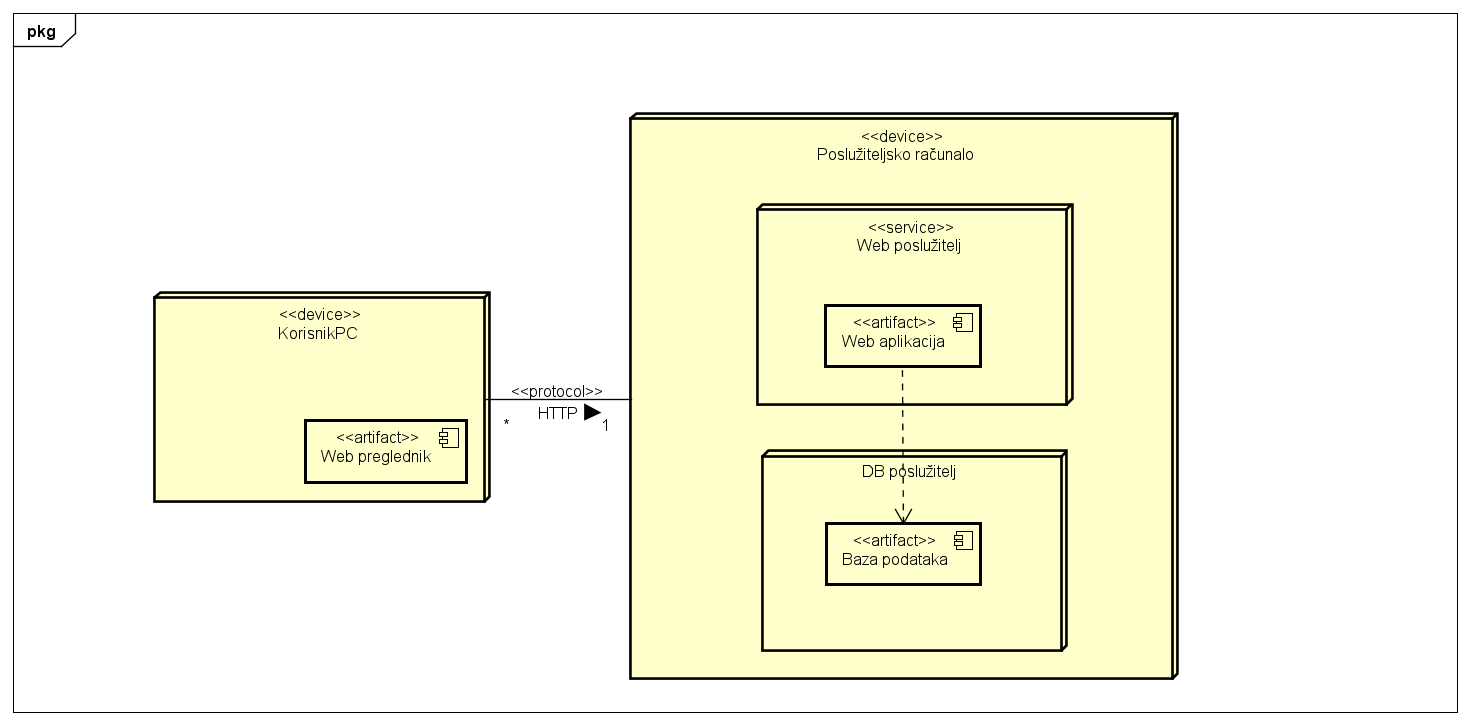
\includegraphics[scale=0.45]{slike/dijagram_razmjestaja.png} %veličina slike u odnosu na originalnu datoteku i pozicija slike
				\centering
				\caption{Dijagram razmještaja}
				\label{fig:promjene}
			\end{figure}
			
			\eject 
		
		\section{Upute za puštanje u pogon}
		
			 
			Za puštanje u pogon korištena je WEB usluga Render istoimene tvrtke, te se puštanje u pogon treba obaviti prema zahtjevima Render platforme. 
			 	
			 \textbf{Konfiguracija poslužitelja baze podataka}
			 
			 Unutar WEB platforme Render potrebno je konfigurirati poslužitelj baze podataka. Na radnoj traci odabiremo opciju new, nakon čega iz padajućeg izbornika treba odabiremo opciju PostgreSQL.
			 
			 
			 \begin{figure}[H]
			 	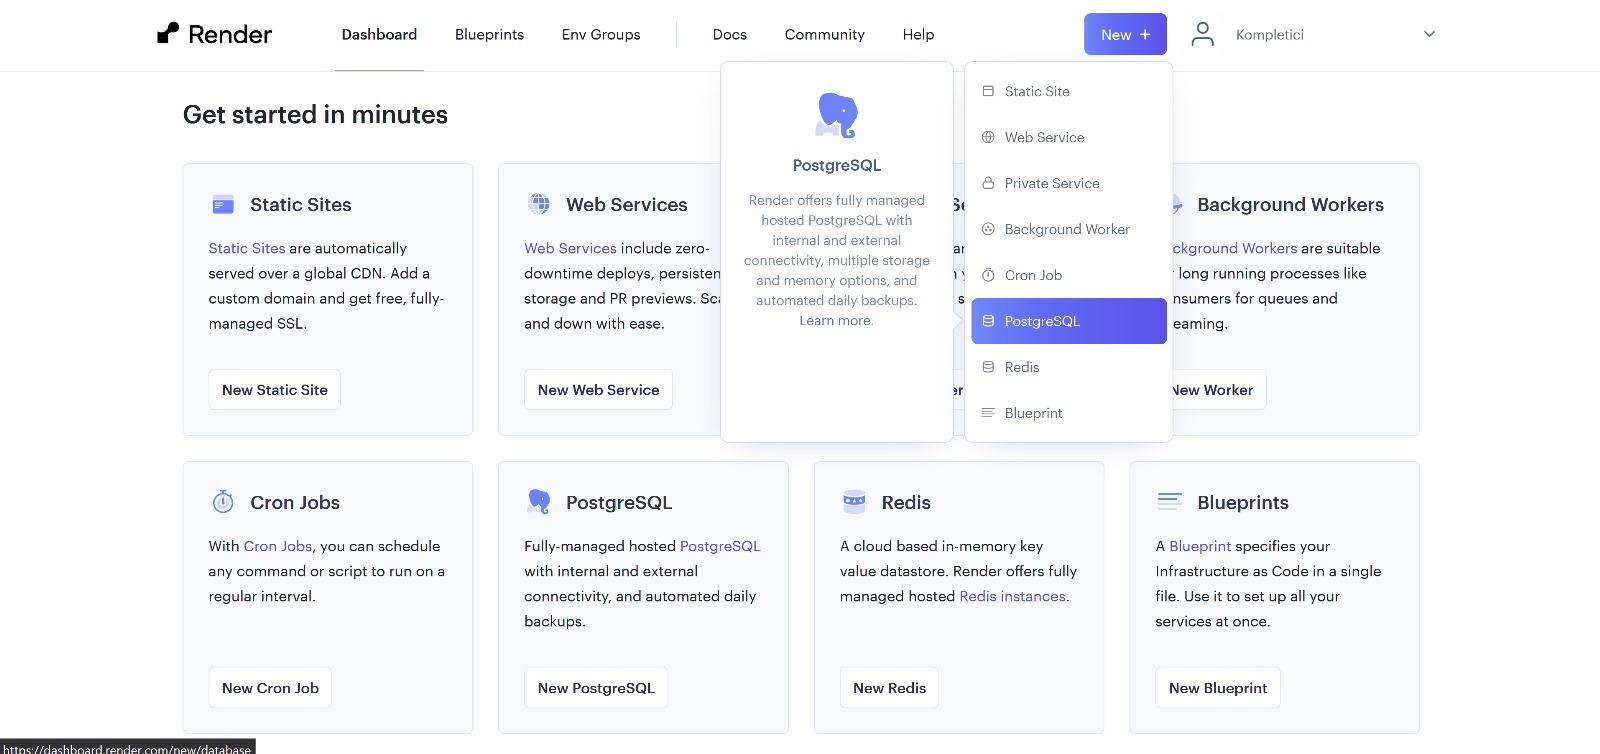
\includegraphics[scale=0.4]{slike/baza_odabir.jpeg} %veličina slike u odnosu na originalnu datoteku i pozicija slike
			 	\centering
			 	\caption{Render korisničko sučelje i radna traka}
			 	\label{fig:promjene}
			 \end{figure}
			 
			 \begin{figure}[H]
			 	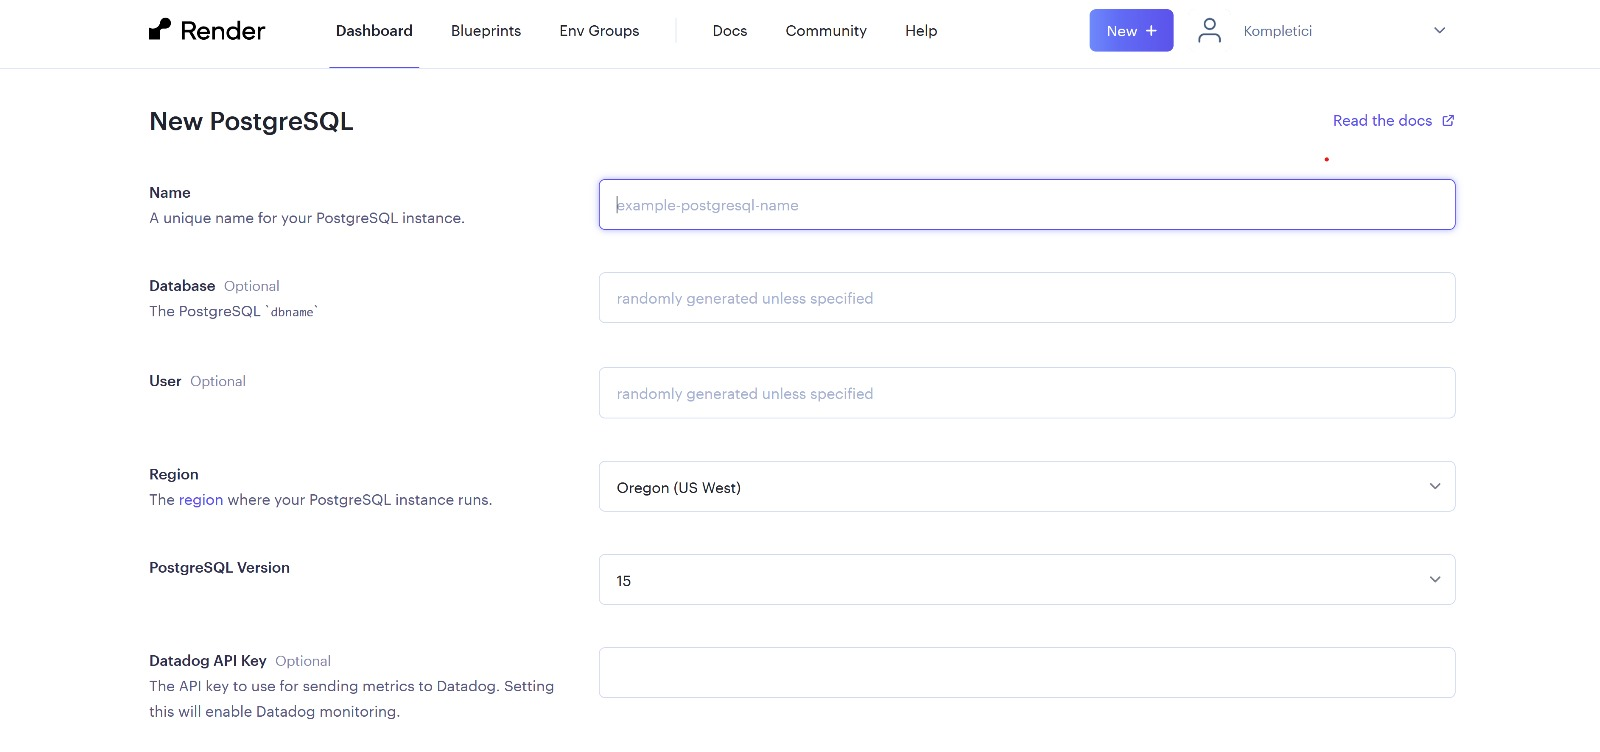
\includegraphics[scale=0.4]{slike/kofiguracija.jpeg} %veličina slike u odnosu na originalnu datoteku i pozicija slike
			 	\centering
			 	\caption{Opcije konfiguracije za bazu podataka}
			 	\label{fig:promjene}
			 \end{figure}
			 
			  Otvoriti će se korisničko sučelje za konfiguraciju baze podataka. Na korisničkom sučelju potrebno je odabrati regiju poslužitelja s kojeg će Render posluživati korisnike. Render će zatim izgenerirati URL poslužitelja baze podataka i lozinku baze podataka, spremamo te podatke jer će nam trebati u daljnjim koracima  

			 \textbf{Konfiguracija backend poslužitelja}
			 
			 Na Render-ovoj radnoj traci odaberemo opciju new WEB service, te odaberemo opciju "Build and deploy from git repository."
			 
			 
			 
			 Nakon toga sljedi proces povezivanja GitHub korisničkog računa i repozitorija s Render korisničkim računom. Potom trebamo odabrati ime za WEB servis te ponovno odabrati regiju poslužitelja s koje će Render posluživati korisnike.
			 
			  \begin{figure}[H]
			 	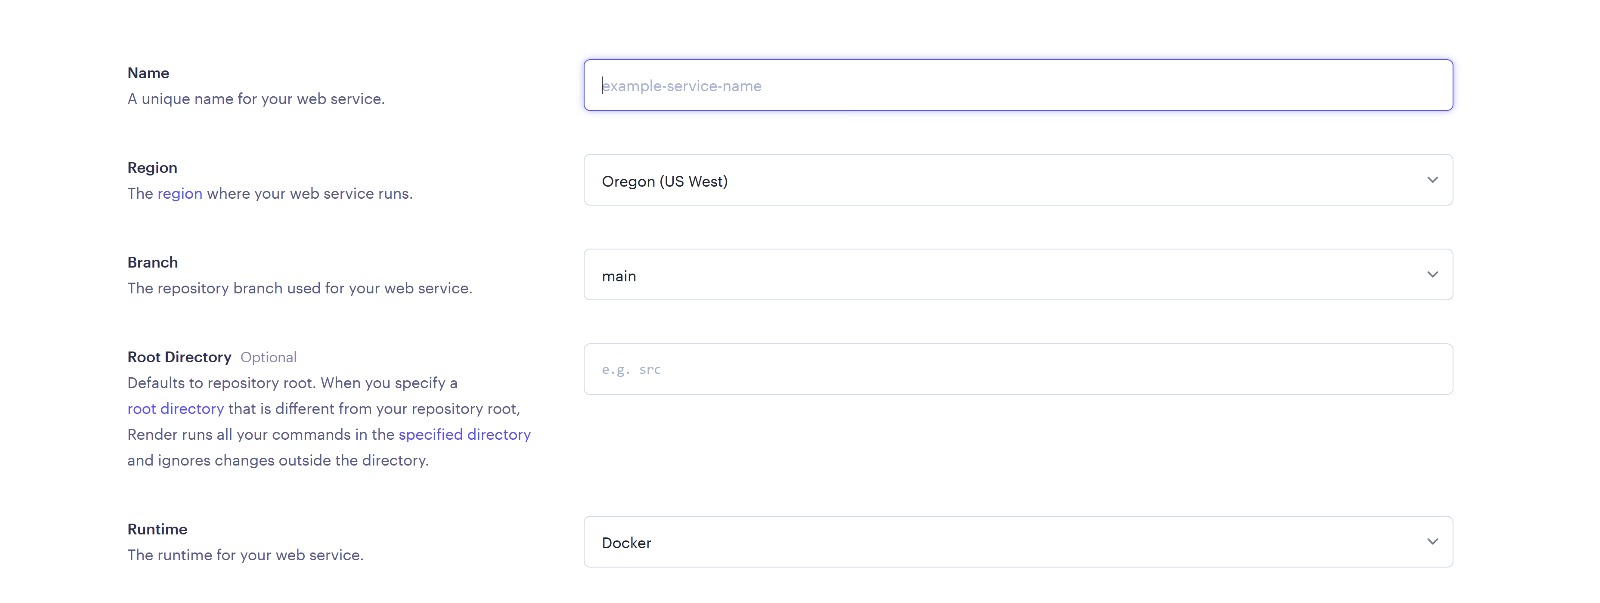
\includegraphics[scale=0.4]{slike/kofiguracija_regije.jpeg} %veličina slike u odnosu na originalnu datoteku i pozicija slike
			 	\centering
			 	\caption{Opcije konfiguracije za WEB servise}
			 	\label{fig:promjene}
			 \end{figure}
			 
			 Nakon toga trebamo odabrati granu GitHub repozitorija s koje će Render povlačiti kod za automatsko puštanje u pogon i odabrati root direktorij backend aplikacije. Za runtime okolinu odabiremo Docker i proširujemo napredne postavke. Dodajemo potrebne varijable okoline poput imena baze, šifre baze i URL baze. Posebnu pozornost trebamo obratiti na format URL-a baze podataka, naime postoji mogućnost da ga treba preoblikovati. On mora biti u sljedećem formatu \textit{\url{jdbc:postgresql://<hostname>:<port>/<database>}}. Konačno moramo dodati putanju Docker datoteke.
			 
			\textbf{Konfiguracija frontend poslužitelja}
			
			
			 Na Renderovoj radnoj traci odabiremo opciju new WEB service, te odabiremo opciju "Build and deploy from git repository." Nakon toga ponovno povezujemo GitHub korisnički račun s Renderom te odabiremo granu koju će Render puštati u pogon. Dodatno odabiremo regiju poslužitelja s kojeg će Render posluživati korisnike. Build komand postavljamo na yarn-build a start komandu na start-prod. Konačno proširujemo napredne postavke te kao varijablu okoline dodajemo adresu deployanog web servisa.
			 
			
			\eject 